\documentclass[UTF8,12pt]{article}
\usepackage{ctex}
\usepackage{indentfirst}
\usepackage{color}
\usepackage{hyperref}
\usepackage{graphicx}
\usepackage{subfigure}
\usepackage{pdfpages}
\usepackage{listings}
\usepackage{afterpage}

\newcommand\myemptypage{
    \null
    \thispagestyle{empty}
    \addtocounter{page}{-1}
    \newpage
}

\hypersetup{
    hidelinks,
	colorlinks=true,
	allcolors=black,
	pdfstartview=Fit,
	breaklinks=true
}

\definecolor{dkgreen}{rgb}{0,0.6,0}
\definecolor{gray}{rgb}{0.5,0.5,0.5}
\definecolor{mauve}{rgb}{0.58,0,0.82}

\lstset{ %
  language=Octave,                % the language of the code
  basicstyle=\footnotesize,           % the size of the fonts that are used for the code
  numbers=left,                   % where to put the line-numbers
  numberstyle=\tiny\color{gray},  % the style that is used for the line-numbers
  stepnumber=2,                   % the step between two line-numbers. If it's 1, each line 
                                  % will be numbered
  numbersep=5pt,                  % how far the line-numbers are from the code
  backgroundcolor=\color{white},      % choose the background color. You must add \usepackage{color}
  showspaces=false,               % show spaces adding particular underscores
  showstringspaces=false,         % underline spaces within strings
  showtabs=false,                 % show tabs within strings adding particular underscores
  frame=single,                   % adds a frame around the code
  rulecolor=\color{black},        % if not set, the frame-color may be changed on line-breaks within not-black text (e.g. commens (green here))
  tabsize=2,                      % sets default tabsize to 2 spaces
  captionpos=b,                   % sets the caption-position to bottom
  breaklines=true,                % sets automatic line breaking
  breakatwhitespace=false,        % sets if automatic breaks should only happen at whitespace
  title=\lstname,                   % show the filename of files included with \lstinputlisting;
                                  % also try caption instead of title
  keywordstyle=\color{blue},          % keyword style
  commentstyle=\color{dkgreen},       % comment style
  stringstyle=\color{mauve},         % string literal style
  escapeinside={\%*}{*)},            % if you want to add LaTeX within your code
  morekeywords={*,...}               % if you want to add more keywords to the set
}


\setlength{\parindent}{2em}

\begin{document}

\begin{titlepage}
    \includepdf[pages={1}]{cover.pdf}
\end{titlepage}

\myemptypage

\begin{center}
    \tableofcontents
\end{center}
\newpage

\section{应用页面设计}
\subsection{Android页面设计技术}
Android系统提供五种常用布局分别为LinearLayout(线性布局)、RelativeLayout(相对布局)、FrameLayout(帧布局)、TableLayout(表格布局)、ConstraintLayout(约束布局)。

\subsubsection{布局的通用属性}
\begin{table}[htbp]
    \centering
    \begin{tabular}{cc}
    \hline
    属性名称                   & 功能描述                 \\ \hline
    android:id             & 设置布局的标识              \\
    android:layout\_width  & 设置布局的宽度              \\
    android:layout\_height & 设置布局的高度              \\
    android:background     & 设置布局的背景              \\
    android:layout\_margin & 设置当前布局与屏幕边界或与周围控件的距离 \\
    android:padding        & 设置当前布局与该布局中控件的距离     \\ \hline
    \end{tabular}
\end{table}

\begin{enumerate}
    \item android:id用于设置当前布局的唯一标识。在XML文件中它的属性值是通过“@+id/属性名称”定义的。为布局指定android:id 属性后,在R.java文件中,会自动生成对应的int值。在Java代码中通过为findViewById()方法传入该int值来获取该布局对象。
    \item android:layout\_width用于设置布局的宽度,其值可以是具体的尺寸,也可以是相对尺寸
    \begin{enumerate}
        \item fill\_parent:表示布局的宽度与父布局的宽度相同
        \item match\_parent:表示布局的宽度与父布局的宽度相同,与fill\_pa
        
        rent相同,在Android 2.2版本后开始推荐使用match\_parent
        \item wrap\_content:表示布局的宽度与当前布局中的控件宽度相同
    \end{enumerate}
    \item android:layout\_height用于设置布局的高度,其值可以是具体的尺寸,也可以是相对尺寸,具体的值与android:layout\_width相同。
    \item android:background用于设置布局的背景,其值可以是颜色值,也可以是图片资源。
    \item android:layout\_margin用于设置当前布局与屏幕边界或与周围控件的距离,其值可以是具体的尺寸,也可以是相对尺寸。与之相似的还有android:paddingTop、android:paddingBottom、android:paddingLeft、android:paddingRight属性,分别用于设置当前布局中控件与该布局上下左右的距离。
\end{enumerate}

需要注意的是,Android系统提供的五种常用布局必须设置android:lay\\out\_width和android:layout\_height属性指定其宽高,其他的属性可以根据需求进行设置。

\subsubsection{LinearLayout(线性布局)}
\begin{table}[htbp]
    \centering
    \begin{tabular}{cc}
    \hline
    \textbf{属性名称}           & \textbf{功能描述}          \\ \hline
    android: oruentation    & 设置布局内控件的排列顺序           \\
    android: layout\_weight & 在布局内设置控件权重,属性值可直接写int值 \\ \hline
    \end{tabular}
\end{table}

\begin{enumerate}
    \item android: oruentation属性用于设置LinearLayout布局中控件的排列顺序,其可选值为vertical和horizontal
    \begin{enumerate}
        \item vertical:表示控件从上到下排列
        \item horizontal:表示控件从左到右排列
    \end{enumerate}
    \item android: layout\_weight属性用于在布局内设置控件权重,属性值可直接写int值,也可以写float值。当android: oruentation属性值为vertical时,android: layout\_weight属性用于设置控件的高度;当android: oruentation属性值为horizontal时,android: layout\_weight属性用于设置控件的宽度。
\end{enumerate}

\subsubsection{RelativeLayout(相对布局)}
\begin{table}[htbp]
    \centering
    \begin{tabular}{cc}
    \hline
    \textbf{属性名称}                     & \textbf{功能描述}        \\ \hline
    android: layout\_centerParent     & 设置当前控件位于父布局的中央位置     \\
    android: layout\_centerVertical   & 设置当前控件位于父布局的垂直居中位置   \\
    android:layout\_centerHorizontal  & 设置当前控件位于父布局的水平居中位置   \\
    android:layout\_above             & 设置当前控件位于某控件上方        \\
    android:layout\_below             & 设置当前控件位于某控件下方        \\
    android:layout\_toLeftOf          & 设置当前控件位于某控件左侧        \\
    android:layout\_toRightOf         & 设置当前控件位于某控件右侧        \\
    android:layout\_alignParentTop    & 设置当前控件是否与父控件顶端对齐     \\
    android:layout\_alignParentLetf   & 设置当前控件是否与父控件左对齐      \\
    android:layout\_alignParentRight  & 设置当前控件是否与父控件右对齐      \\
    android:layout\_alignParentBottom & 设置当前控件是否与父控件底端对齐     \\
    android:layout\_alignTop          & 设置当前控件的上边界与某控件的上边界对齐 \\
    android:layout\_alignBottom       & 设置当前控件的下边界与某控件的下边界对齐 \\
    android:layout\_alignLeft         & 设置当前控件的左边界与某控件的左边界对齐 \\
    android:layout\_alignRight        & 设置当前控件的右边界与某控件的右边界对齐 \\ \hline
    \end{tabular}
\end{table}

\subsubsection{FrameLayout(帧布局)}
FrameLayout(帧布局)用于在屏幕上创建一块空白区域,添加到该区域中的每个子控件占一帧,这些帧会一个一个叠加在一起,后加入的控件会叠加在上一个控件上层。默认情况下,帧布局中的所有控件会与左上角对齐。

\begin{table}[htbp]
    \centering
    \begin{tabular}{cc}
    \hline
    \textbf{属性名称}              & \textbf{功能描述}            \\ \hline
    android: foreground        & 设置帧布局容器的前景图像(始终在所有子控件之上) \\
    android: foregroundGravity & 设置前景图像显示的位置              \\ \hline
    \end{tabular}
\end{table}

\subsubsection{TableLayout(表格布局)}
TableLayout(表格布局)采用行、列的形式来管理控件,它不需要明确声明包含多少行、多少列,而是通过在TableLayout(表格布局)中添加TableLayout(表格布局)或控件来控制表格的行数,可以在TableRow布局中添加控件来控制表格的列数。

\begin{table}[htbp]
    \centering
    \begin{tabular}{cc}
    \hline
    属性名称                    & 功能描述            \\ \hline
    android:stretchColumns  & 设置可被拉伸的列        \\
    android:shrinkColumns   & 设置可被收缩的列        \\
    android:collapseColumns & 设置可被隐藏的列        \\
    android:layout\_column  & 设置该控件显示的位置      \\
    android:layout\_span    & 设置该控件占据几行,默认为1行 \\ \hline
    \end{tabular}
\end{table}

\subsubsection{ConstraintLayout(约束布局)}
ConstraintLayout(约束布局)是Android Studio 2.2新添加的布局。与前介绍的界面布局相比,ConstraintLayout(约束布局)并不太适合使用XML代码的方法编写布局,但是它非常适合使用可视化的方式编写界面布局。实践不采用可视化方式编写界面,因此这里不展开介绍。

\subsection{界面跳转流程图}
\begin{figure}[htbp]
    \centering
    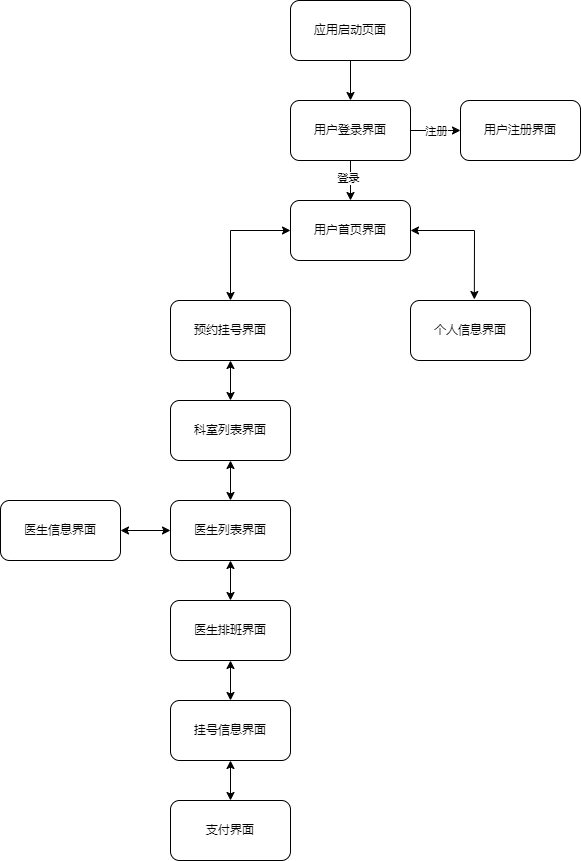
\includegraphics[width=0.9\textwidth]{imgs/1.png}
    \caption{界面跳转流程图}
    \label{fig:flowchart}
\end{figure}

\newpage

共计12个界面

\subsection{具体页面设计}
\subsubsection{启动界面}
在程序启动的时候,需要一个启动界面,用于展示程序的logo,同时在启动界面中进行一些初始化操作,设置3s自动关闭启动界面。启动界面并不需要做的很复杂,只需要设计一个背景,然后添加一个按钮用于跳过启动界面即可。

设计的XML代码如下:

\begin{lstlisting}
<?xml version="1.0" encoding="utf-8"?>
<RelativeLayout xmlns:android="http://schemas.android.com/apk/res/android"
    xmlns:app="http://schemas.android.com/apk/res-auto"
    xmlns:tools="http://schemas.android.com/tools"
    android:layout_width="match_parent"
    android:layout_height="match_parent"
    tools:context=".ui.activity.SplashActivity"
    android:background="@mipmap/splashbg">
    <Button
        android:id="@+id/id_btn_skip"
        android:layout_alignParentRight="true"
        android:layout_alignParentTop="true"
        android:layout_width="wrap_content"
        android:layout_height="wrap_content"
        android:layout_gravity="right"
        android:layout_marginRight="32dp"
        android:layout_marginTop="32dp"
        android:background="@drawable/btn_bg_skip"
        android:paddingBottom="4dp"
        android:paddingLeft="12dp"
        android:paddingRight="12dp"
        android:paddingTop="4dp"
        android:text="跳过"
        android:minWidth="0dp"
        android:minHeight="0dp"
        android:textColor="#ffffff"
        android:textSize="14sp" />
</RelativeLayout>
\end{lstlisting}

界面效果如下:

\begin{figure}[htbp]
    \centering
    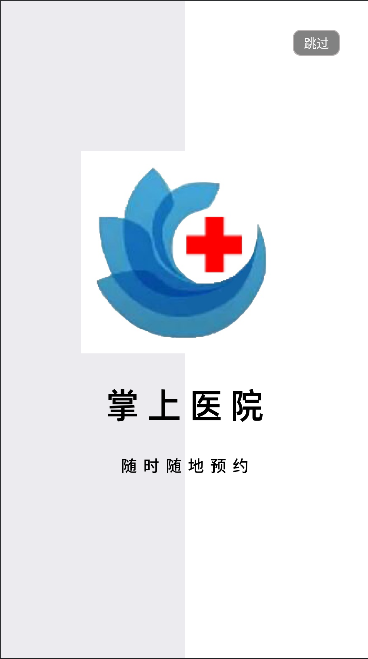
\includegraphics[width=0.5\textwidth]{imgs/2.png}
    \caption{启动界面}
    \label{fig:splash}
\end{figure}

\subsubsection{登录界面}
登录界面需要设计一个背景,然后添加一个logo,接着添加两个输入框,分别用于输入用户名和密码,最后添加一个登录按钮。需要注意的是,在登录界面需要额外设置一个按钮,用于跳转到注册界面。
\begin{lstlisting}
<?xml version="1.0" encoding="utf-8"?>
<RelativeLayout xmlns:android="http://schemas.android.com/apk/res/android"
    xmlns:app="http://schemas.android.com/apk/res-auto"
    xmlns:tools="http://schemas.android.com/tools"
    android:layout_width="match_parent"
    android:layout_height="match_parent"
    tools:context=".ui.activity.LoginActivity"
    android:background="@mipmap/login_bg">
    <TextView
        android:id="@+id/id_tv_title"
        android:layout_width="wrap_content"
        android:layout_height="wrap_content"
        android:layout_centerHorizontal="true"
        android:layout_marginTop="90dp"
        android:text="掌上医院"
        android:textSize="40sp"
        android:textStyle="bold"></TextView>
    <EditText
        android:paddingLeft="20dp"
        android:id="@+id/id_et_uid"
        android:layout_width="match_parent"
        android:layout_height="56dp"
        android:layout_below="@id/id_tv_title"
        android:layout_marginTop="40dp"
        android:background="#44ffffff"
        android:hint="请输入账号"
        android:inputType="text"
        android:textColorHint="#070707" />
    <EditText
        android:paddingLeft="20dp"
        android:id="@+id/id_et_upsw"
        android:layout_width="match_parent"
        android:layout_height="56dp"
        android:layout_below="@id/id_et_uid"
        android:layout_marginTop="4dp"
        android:background="#44ffffff"
        android:hint="请输入密码"
        android:inputType="textWebPassword"
        android:textColorHint="#070707" />
    <Button
        android:id="@+id/id_btn_login"
        android:layout_width="match_parent"
        android:layout_height="wrap_content"
        android:layout_below="@id/id_et_upsw"
        android:layout_marginLeft="60dp"
        android:layout_marginTop="50dp"
        android:layout_marginRight="60dp"
        android:background="#87CEFA"
        android:text="登录"
        android:textSize="26sp" />
    <TextView
        android:id="@+id/id_tv_register"
        android:layout_width="wrap_content"
        android:layout_height="wrap_content"
        android:layout_below="@id/id_btn_login"
        android:layout_centerHorizontal="true"
        android:layout_marginTop="30dp"
        android:text="注册账号"
        android:textSize="18sp"
        android:textColor="#000000" />
</RelativeLayout>
\end{lstlisting}

以上是登录界面的XML代码,界面效果如下:

\begin{figure}[htbp]
    \centering
    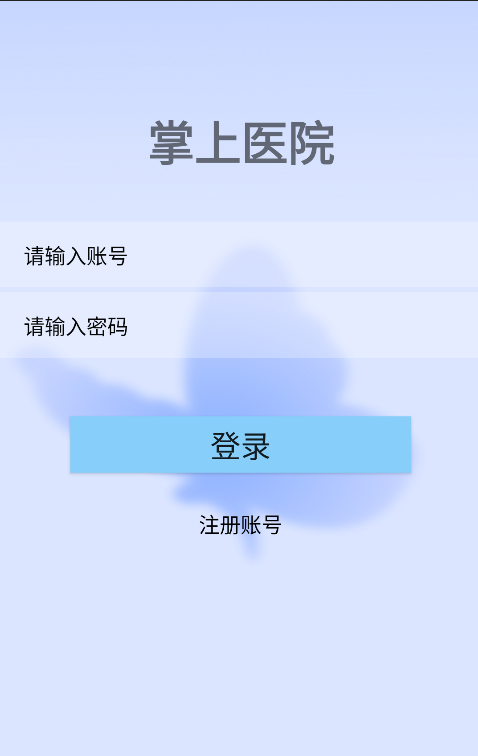
\includegraphics[width=0.3\textwidth]{imgs/3.png}
    \caption{登录界面}
    \label{fig:login}
\end{figure}

\subsubsection{注册界面}
注册界面需要设计一个背景,然后添加一个logo,接着添加四个输入框,分别用于输入用户姓名、用户名、密码、重复密码,最后添加一个注册按钮。需要注意的是,在注册界面需要额外设置一个按钮,用于跳转到登录界面。

这里的XML源码比较长,不进行展示,界面效果如下:

\begin{figure}[htbp]
    \centering
    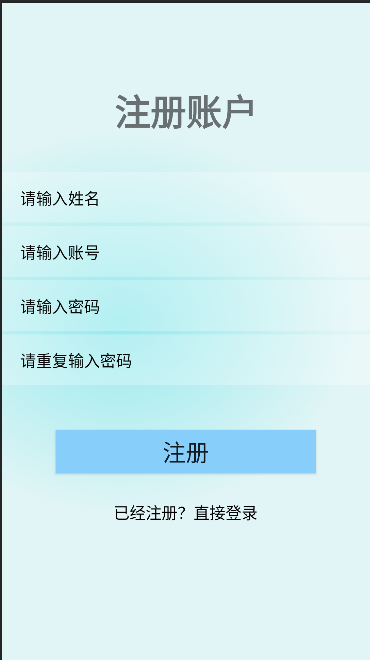
\includegraphics[width=0.2\textwidth]{imgs/4.png}
    \caption{注册界面}
    \label{fig:register}
\end{figure}



\subsubsection{用户首页}
用户首页设置一个背景,然后添加一个logo,接着添加三个按钮,分别用于跳转到预约挂号、我的信息、退出登录。目前只对用户首页进行了简单设计,并没有添加美化内容,只展示一个原型界面

实现的XML代码如下:

\begin{lstlisting}
    <?xml version="1.0" encoding="utf-8"?>
    <LinearLayout
        xmlns:android="http://schemas.android.com/apk/res/android"
        xmlns:app="http://schemas.android.com/apk/res-auto"
        xmlns:tools="http://schemas.android.com/tools"
        android:layout_width="match_parent"
        android:layout_height="match_parent"
        android:orientation="vertical"
        tools:context=".ui.activity.IndexActivity"
        android:background="@mipmap/login_bg"
    
        >
        <TextView
            android:id="@+id/welcome_uname"
            android:layout_marginTop="30dp"
            android:layout_width="match_parent"
            android:layout_height="50dp"
            android:text="李明,欢迎您!"
            android:gravity="center"
            android:textSize="26sp"
            android:textColor="@color/black"
            ></TextView>
        <Button
            android:id="@+id/btn1"
            android:layout_width="match_parent"
            android:layout_height="wrap_content"
            android:text="预约挂号"
            android:layout_marginTop="30dp"
            android:layout_marginLeft="20dp"
            android:layout_marginRight="20dp"
            android:textSize="26sp"
            android:background="#87CEFA"
            />
    
        <Button
            android:id="@+id/btn2"
            android:layout_width="match_parent"
            android:layout_height="wrap_content"
            android:text="我的信息"
    
            android:layout_marginTop="50dp"
            android:layout_marginLeft="20dp"
            android:layout_marginRight="20dp"
            android:textSize="26sp"
            android:background="#87CEFA"/>
        <Button
            android:id="@+id/btn3"
            android:layout_width="match_parent"
            android:layout_height="wrap_content"
            android:text="退出账号"
    
            android:layout_marginTop="50dp"
            android:layout_marginLeft="20dp"
            android:layout_marginRight="20dp"
            android:textSize="26sp"
            android:background="#87CEFA"/>
    </LinearLayout>
\end{lstlisting}

界面效果如下:

\newpage

\begin{figure}[htbp]
    \centering
    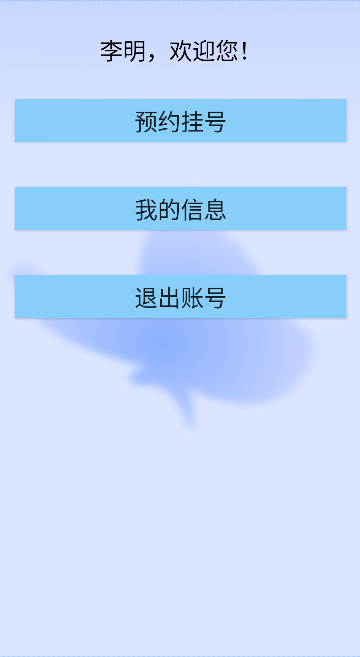
\includegraphics[width=0.5\textwidth]{imgs/5.png}
    \caption{用户首页}
    \label{fig:index}
\end{figure}

用户在预约挂号时,展现的科室列表、医生列表实际是一致的,在顶部标题处作区分,这里只展示科室列表设计。

\subsubsection{科室列表}
科室列表是一个列表,需要设计一个背景,然后添加一个logo,接着添加一个列表,用于展示科室列表

实现的XML代码如下:

\newpage

\begin{lstlisting}
<?xml version="1.0" encoding="utf-8"?>
<LinearLayout xmlns:android="http://schemas.android.com/apk/res/android"
    xmlns:app="http://schemas.android.com/apk/res-auto"
    xmlns:tools="http://schemas.android.com/tools"
    android:layout_width="match_parent"
    android:layout_height="match_parent"
    tools:context=".ui.activity.ChooseDepartActivity"
    android:orientation="vertical">
    <LinearLayout
        android:layout_width="wrap_content"
        android:layout_height="40dp">
        <ImageView
            android:id="@+id/btn_back"
            android:layout_width="40dp"
            android:layout_height="40dp"
            android:src="@mipmap/btn_back"></ImageView>
    </LinearLayout>
    <ListView
        android:id="@+id/depart_list_view"
        android:layout_width="match_parent"
        android:layout_height="match_parent"
        android:layout_marginLeft="20dp"
        android:layout_marginRight="20dp"></ListView>
</LinearLayout>
\end{lstlisting}

在列表的顶部作区分,部门、医生列表的顶部没有特殊设计,排班时间选择的时候,顶部打印了当前选择的医生信息。

以上就是当前设计的界面部分,后续还会继续添加,这里不再一一展示。




\end{document}